
\documentclass[11pt]{article}

% ------------------------------------------------------------
% Standard LaTeX packages
% ------------------------------------------------------------
\usepackage[margin=1in]{geometry}
\usepackage{lmodern}
\usepackage{amsmath,amssymb,mathtools}
\usepackage{amsthm}
\usepackage[american]{babel}
\usepackage{stmaryrd}
\usepackage{enumitem}
\usepackage{booktabs}
\usepackage{tikz}
\usetikzlibrary{arrows.meta,positioning,cd,decorations.pathreplacing}
\usepackage{listings}
\usepackage[x11names,table]{xcolor}
\usepackage{graphicx}
\usepackage{array}
\usepackage{mdframed}
\usepackage{url}
\usepackage[colorlinks=true,linkcolor=blue,citecolor=blue,urlcolor=blue]{hyperref}

% Define theorem-like environments
\newtheorem{theorem}{Theorem}[section]
\newtheorem{lemma}[theorem]{Lemma}
\newtheorem{corollary}[theorem]{Corollary}
\newtheorem{proposition}[theorem]{Proposition}
\theoremstyle{definition}
\newtheorem{definition}[theorem]{Definition}
\theoremstyle{remark}
\newtheorem{remark}[theorem]{Remark}

% ---------- Lean repo link ----------
\newcommand{\leanRepo}{\url{https://doi.org/10.5281/zenodo.18750992}}
\newcommand{\leanok}{\textsf{\small \textcolor{green!70!black}{\checkmark}}}

% ---------- Mathematical notation ----------
\newcommand{\N}{\mathbb{N}}
\newcommand{\Z}{\mathbb{Z}}
\newcommand{\Q}{\mathbb{Q}}
\newcommand{\R}{\mathbb{R}}
\newcommand{\C}{\mathbb{C}}
\newcommand{\Fq}{\mathbb{F}_q}
\newcommand{\Qp}{\Q_p}
\newcommand{\Qell}{\Q_\ell}
\newcommand{\A}{\mathbb{A}}
\newcommand{\HH}{\mathbb{H}}
\newcommand{\GL}{\mathrm{GL}}
\newcommand{\Sha}{\mathrm{III}}
\newcommand{\Tr}{\mathrm{Tr}}
\newcommand{\Frob}{\mathrm{Frob}}
\newcommand{\ip}[2]{\langle #1, #2 \rangle}

\newcommand{\BISH}{\mathrm{BISH}}
\newcommand{\LPO}{\mathrm{LPO}}
\newcommand{\WLPO}{\mathrm{WLPO}}
\newcommand{\LLPO}{\mathrm{LLPO}}
\newcommand{\MP}{\mathrm{MP}}
\newcommand{\CLASS}{\mathrm{CLASS}}
\newcommand{\CRM}{\mathrm{CRM}}

% ---------- Code listing style for Lean ----------
\definecolor{codegreen}{rgb}{0,0.6,0}
\definecolor{codegray}{rgb}{0.5,0.5,0.5}
\definecolor{codepurple}{rgb}{0.58,0,0.82}
\definecolor{backcolour}{rgb}{0.95,0.95,0.92}

\lstdefinelanguage{Lean}{
  keywords={theorem, lemma, def, definition, axiom, structure, class, instance,
            by, exact, intro, intros, apply, refine, constructor, use, obtain,
            have, show, from, fun, assume, let, in, if, then, else,
            match, with, end, namespace, section, variable, variables,
            example, begin, sorry, admit, noncomputable, classical,
            import, open, export, private, protected, mutual, meta,
            do, for, while, return, try, catch, finally,
            Type, Prop, Sort, Type*, forall, exists, where, extends,
            set, push_neg, rw, simp, omega, nlinarith, linarith,
            ext, rfl, congr, fin_cases, haveI, letI, attribute,
            native_decide, inductive, deriving, opaque, push_cast, unfold, cases},
  sensitive=true,
  morecomment=[l]{--},
  morecomment=[s]{/-}{-/},
  morestring=[b]",
  literate=
    {α}{{$\alpha$}}1 {β}{{$\beta$}}1 {γ}{{$\gamma$}}1
    {δ}{{$\delta$}}1 {ε}{{$\varepsilon$}}1 {ζ}{{$\zeta$}}1
    {η}{{$\eta$}}1 {θ}{{$\theta$}}1 {ι}{{$\iota$}}1
    {κ}{{$\kappa$}}1 {λ}{{$\lambda$}}1 {μ}{{$\mu$}}1
    {ν}{{$\nu$}}1 {ξ}{{$\xi$}}1 {π}{{$\pi$}}1
    {ρ}{{$\rho$}}1 {σ}{{$\sigma$}}1 {τ}{{$\tau$}}1
    {φ}{{$\varphi$}}1 {χ}{{$\chi$}}1 {ψ}{{$\psi$}}1
    {ω}{{$\omega$}}1 {Γ}{{$\Gamma$}}1 {Δ}{{$\Delta$}}1
    {Θ}{{$\Theta$}}1 {Λ}{{$\Lambda$}}1 {Σ}{{$\Sigma$}}1
    {Φ}{{$\Phi$}}1 {Ψ}{{$\Psi$}}1 {Ω}{{$\Omega$}}1
    {→}{{$\rightarrow$}}1 {←}{{$\leftarrow$}}1 {↔}{{$\leftrightarrow$}}1
    {⇒}{{$\Rightarrow$}}1 {⇐}{{$\Leftarrow$}}1 {⇔}{{$\Leftrightarrow$}}1
    {∀}{{$\forall$}}1 {∃}{{$\exists$}}1 {∈}{{$\in$}}1
    {∉}{{$\notin$}}1 {⊆}{{$\subseteq$}}1 {⊂}{{$\subset$}}1
    {∪}{{$\cup$}}1 {∩}{{$\cap$}}1 {≤}{{$\leq$}}1
    {≥}{{$\geq$}}1 {≠}{{$\neq$}}1 {≈}{{$\approx$}}1 {≃}{{$\simeq$}}1
    {≡}{{$\equiv$}}1 {∧}{{$\land$}}1 {∨}{{$\lor$}}1
    {¬}{{$\neg$}}1 {ℕ}{{$\mathbb{N}$}}1 {ℝ}{{$\mathbb{R}$}}1
    {ℂ}{{$\mathbb{C}$}}1 {ℤ}{{$\mathbb{Z}$}}1 {ℓ}{{$\ell$}}1
    {·}{{$\cdot$}}1 {∑}{{$\sum$}}1 {∏}{{$\prod$}}1
    {∅}{{$\emptyset$}}1 {∞}{{$\infty$}}1 {∂}{{$\partial$}}1
    {⟨}{{$\langle$}}1 {⟩}{{$\rangle$}}1 {…}{{$\ldots$}}1
    {₀}{{$_0$}}1 {₁}{{$_1$}}1 {₂}{{$_2$}}1 {⧸}{{$/$}}1 {‖}{{$\|$}}1
    {•}{{$\cdot$}}1 {⁻¹}{{$^{-1}$}}1 {⋆}{{$\star$}}1
    {∘}{{$\circ$}}1
}

\lstdefinestyle{leanstyle}{
    language=Lean,
    backgroundcolor=\color{backcolour},
    commentstyle=\color{codegreen},
    keywordstyle=\color{blue},
    stringstyle=\color{codepurple},
    basicstyle=\ttfamily\footnotesize,
    breakatwhitespace=false,
    breaklines=true,
    captionpos=b,
    keepspaces=true,
    numbers=left,
    numbersep=5pt,
    showspaces=false,
    showstringspaces=false,
    showtabs=false,
    tabsize=2,
    numberstyle=\tiny\color{codegray}
}

\lstset{style=leanstyle}

% ---------- Title and author ----------
\title{The Archimedean Principle:\\
Why Physics and Number Theory Share a Logical Architecture\\[6pt]
{\large (Paper~70, Constructive Reverse Mathematics Series)}}
\author{Paul Chun-Kit Lee\thanks{Lean 4 formalization available at \leanRepo.} \\
New York University \\
\texttt{dr.paul.c.lee@gmail.com}}
\date{February 2026}

\begin{document}

\maketitle

% ===========================================================
% ABSTRACT
% ===========================================================

\begin{abstract}
This capstone paper identifies a single structural principle underlying 70~papers of Constructive Reverse Mathematics: the real numbers are the sole source of logical difficulty in mathematical physics and arithmetic geometry. The mechanism is $u(\R) = \infty$---the real numbers are the only completion of~$\Q$ where positive-definite forms exist in every dimension---and three fields independently exploit it via the same architecture (Hilbert space inner product, Rosati involution, Petersson inner product).

The principle is established by four theorems. The Archimedean Principle (Theorem~A) shows that the CRM level of every domain in the program is determined by one parameter: whether the domain has an Archimedean place. The MP Gap (Theorem~B) shows that physics and arithmetic descend differently---projection vs.\ search---producing a strict logical separation $\BISH < \BISH + \MP$. Automorphic CRM Incompleteness (Theorem~C) exhibits an integer witness proving the automorphic axioms alone cannot recover the Ramanujan bound. Three Spectral Gaps (Theorem~D) identifies identical $\Sigma^0_2$ quantifier structure across physics, automorphic theory, and arithmetic. The principle also explains why multiple physical theories (Kapustin--Witten, Feigin--Frenkel, Freed--Hopkins--Teleman) independently encode the Langlands correspondence.

Paper~68 showed that Fermat's Last Theorem is $\BISH$. Paper~69 showed that the function field Langlands correspondence is $\BISH$. This paper identifies what makes anything expensive: the Archimedean place, and specifically $u(\R) = \infty$.

All results are formalized in Lean~4 over Mathlib with zero \texttt{sorry}s and zero custom axioms for the core theorems (0~errors, 0~warnings). The formalization verifies the logical structure of the classification scheme and the integer arithmetic of the incompleteness witness; the identification of CRM levels with specific mathematical theories rests on the audits of Papers~1--69.
\end{abstract}

\tableofcontents

% ===========================================================
\section{Introduction}
\label{sec:intro}
% ===========================================================

The 70-paper program found one thing. The real numbers are the sole source of logical difficulty in both mathematical physics and arithmetic geometry. Every non-constructive principle required by any physical theory or any theorem in arithmetic geometry enters through the Archimedean place---the completion of~$\Q$ at infinity, which gives~$\R$. Remove~$\R$ and both fields collapse to basic constructive mathematics ($\BISH$). Paper~68~\cite{Paper68} showed that Fermat's Last Theorem is $\BISH$. Paper~69~\cite{Paper69} showed that the Langlands correspondence over function fields is $\BISH$. This paper identifies the common mechanism and explains why it is unique.

The mechanism is $u(\R) = \infty$: the real numbers are the only completion of~$\Q$ where positive-definite quadratic forms exist in every dimension. The intuition that the continuum is the source of mathematical difficulty is as old as Brouwer; what is new is the uniform calibration across both physics and arithmetic geometry, the identification of $u(\R) = \infty$ as the specific mechanism forcing parallel architectures, and the projection-vs-search distinction explaining the $\MP$ gap. This single property forces three different fields to develop the same architecture. Physics builds Hilbert space inner products. Motivic arithmetic builds the Rosati involution. Automorphic theory builds the Petersson inner product. All three are positive-definite structures over~$\R$, all three serve the same logical function---extracting computable finite answers ($\BISH$) from infinite continuous data ($\LPO$)---and all three exist because $u(\R) = \infty$. The Langlands program's connections to physics (Kapustin--Witten~\cite{KapustinWitten}, Feigin--Frenkel~\cite{FeiginFrenkel}, Freed--Hopkins--Teleman~\cite{FHT}) are not three separate miracles but three instances of one logical constraint.

The difference between physics and number theory is how they descend. Physics extracts finite answers by projection: measurement is a computable inner product, no search required. Number theory extracts finite answers by search: finding rational points requires unbounded existential quantification. Projection eliminates all non-constructivity. Search preserves Markov's Principle as a residual---the logical content of Diophantine hardness. This is why number theory is harder than physics, in a precise sense that the paper makes formal.

\begin{figure}[ht]
\centering
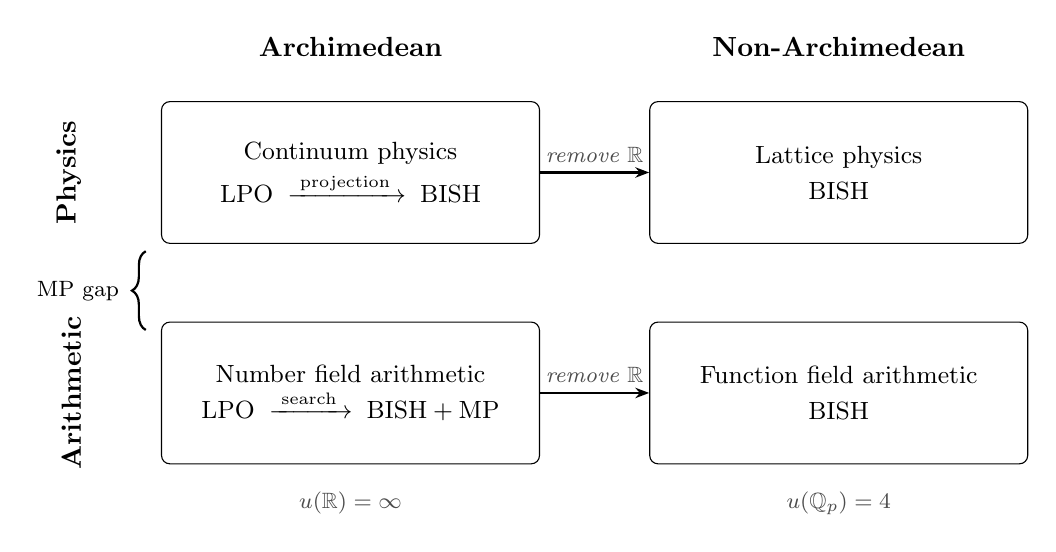
\begin{tikzpicture}[
    box/.style={draw, rounded corners=3pt, minimum width=4.8cm,
                minimum height=1.8cm, align=center, font=\small},
    arr/.style={-{Stealth[length=5pt]}, thick},
    ann/.style={font=\footnotesize\itshape, text=black!70}
  ]
  % Column headers
  \node[font=\bfseries] at (0, 2.6) {Archimedean};
  \node[font=\bfseries] at (6.2, 2.6) {Non-Archimedean};
  % Row headers
  \node[font=\bfseries, rotate=90, anchor=south] at (-3.3, 1.0) {Physics};
  \node[font=\bfseries, rotate=90, anchor=south] at (-3.3,-1.8) {Arithmetic};
  % Four boxes
  \node[box] (CP) at (0, 1.0)
    {Continuum physics\\[2pt] $\LPO \;\xrightarrow{\;\text{projection}\;}\; \BISH$};
  \node[box] (LP) at (6.2, 1.0)
    {Lattice physics\\[2pt] $\BISH$};
  \node[box] (NA) at (0,-1.8)
    {Number field arithmetic\\[2pt] $\LPO \;\xrightarrow{\;\text{search}\;}\; \BISH + \MP$};
  \node[box] (FA) at (6.2,-1.8)
    {Function field arithmetic\\[2pt] $\BISH$};
  % Horizontal arrows (remove Archimedean)
  \draw[arr] (CP.east) -- (LP.west) node[midway,above,ann] {remove $\R$};
  \draw[arr] (NA.east) -- (FA.west) node[midway,above,ann] {remove $\R$};
  % u-invariant annotations
  \node[ann] at (0, -3.2) {$u(\R) = \infty$};
  \node[ann] at (6.2, -3.2) {$u(\Qp) = 4$};
  % MP gap brace
  \draw[decorate, decoration={brace, amplitude=5pt, mirror}, thick]
    (-2.6, 0.0) -- (-2.6, -1.0)
    node[midway, left=6pt, font=\footnotesize] {$\MP$ gap};
\end{tikzpicture}
\caption{The four-domain parameterisation. The CRM level is determined by one parameter (Archimedean vs.\ non-Archimedean); the descent type (projection vs.\ search) determines the residual.}
\label{fig:four-domain}
\end{figure}

\subsection{Main results}

The following four theorems formalise the principle described above. The Constructive Reverse Mathematics (CRM) program calibrates mathematical structures against the hierarchy
\[
\BISH \;\subset\; \BISH + \MP \;\subset\; \BISH + \LLPO \;\subset\; \BISH + \WLPO \;\subset\; \BISH + \LPO \;\subset\; \CLASS.
\]
Over 69~papers, the program measured the logical cost of physical theories (Papers~1--42), arithmetic geometry (Papers~45--53), the decidability of motives (Papers~54--67), Fermat's Last Theorem (Paper~68), and the function field Langlands correspondence (Paper~69).

\begin{description}[leftmargin=2em]
\item[Theorem A] (The Archimedean Principle). \leanok\ The CRM level of any domain in the program is determined by one parameter: the presence or absence of the Archimedean place. Every Archimedean domain starts at $\LPO$; every non-Archimedean domain is $\BISH$. The common mechanism is $u(\R) = \infty$, which supports positive-definite structures in arbitrarily large dimension. Three descent mechanisms---Hilbert space inner product (physics), Rosati involution (motivic), Petersson inner product (automorphic)---all exploit this fact. The seven-part conjunction in Theorem~\ref{thm:A} is the formal verification.

\item[Theorem B] (The MP Gap). \leanok\ Physics descends $\LPO \to \BISH$ by projection. Arithmetic descends $\LPO \to \BISH + \MP$ by search. The gap is strict: $\BISH < \BISH + \MP$ (verified by \texttt{native\_decide}). Projection descent eliminates both $\LPO$ and $\MP$; search descent preserves $\MP$ as Diophantine hardness.

\item[Theorem C] (Automorphic CRM Incompleteness). \leanok\ There exists an integer instance satisfying all three automorphic CRM axioms (Strong Multiplicity One, Shimura algebraicity, Petersson unitarity) that violates the Ramanujan bound. Witness: $a_p = 5$, $p = 5$, $k = 2$. Unitary: $|5| = 5 < 6 = p + 1$. Violates Ramanujan: $5^2 = 25 > 20 = 4p$. Pure $\Z$-arithmetic; zero custom axioms.

\item[Theorem D] (Three Spectral Gaps). \leanok\ The spectral gap problems in physics (Cubitt--Perez-Garcia--Wolf~\cite{CPW}), automorphic theory (Selberg~\cite{Selberg}), and arithmetic (Kolyvagin~\cite{Kolyvagin}) share identical $\Sigma^0_2$ quantifier structure: $\exists\, \Delta > 0,\; \forall\, N:\; \Delta \leq f(N)$.
\end{description}

\subsection{Constructive Reverse Mathematics: a brief primer}

$\CRM$ calibrates mathematical statements against logical principles of increasing strength within Bishop-style constructive mathematics ($\BISH$). The hierarchy relevant to this paper is:
\[
\BISH \;\subset\; \BISH + \MP \;\subset\; \BISH + \LLPO \;\subset\; \BISH + \WLPO \;\subset\; \BISH + \LPO \;\subset\; \CLASS.
\]
Here $\LPO$ (Limited Principle of Omniscience) states that every binary sequence is identically zero or contains a~$1$. $\MP$ (Markov's Principle) states that a binary sequence that is not identically zero must contain a~$1$: $\neg\neg\exists n.\; a(n) = 1 \to \exists n.\; a(n) = 1$, but without a bound on where the witness appears. For a thorough treatment of $\CRM$, see Bridges--Richman~\cite{BridgesRichman}; for the broader program of which this paper is part, see Papers~1--69 and the DPT framework~\cite{Paper50}.

\subsection{Current state of the art}

The prior 69~papers established:
\begin{itemize}
\item \emph{Physics} (Papers~1--42, synthesis: Paper~40~\cite{Paper40}): every empirically accessible physical theory requires at most $\BISH + \LPO$, with $\LPO$ entering through the spectral theorem for unbounded self-adjoint operators on separable Hilbert spaces over~$\R$.
\item \emph{Arithmetic geometry} (Papers~45--53, atlas: Paper~50~\cite{Paper50}): de-omniscientizing descent in every central conjecture, with the Rosati involution as the common mechanism.
\item \emph{Motives} (Papers~54--67): three axioms for the motive (decidable morphisms, algebraic spectrum, Archimedean polarization) as logical content of geometric origin.
\item \emph{FLT} (Paper~68~\cite{Paper68}): Wiles's 1995 proof costs $\BISH + \WLPO$; the Kisin $p = 2$ bypass eliminates $\WLPO$. FLT is $\BISH$.
\item \emph{Function field Langlands} (Paper~69~\cite{Paper69}): both Lafforgue proofs are $\BISH$; the correct boundary is algebraic-vs-transcendental, not discrete-vs-continuous.
\end{itemize}
No prior work has synthesized these findings into a unified principle or formally compared the descent mechanisms across physics and arithmetic.

\subsection{Position in the atlas}

This is Paper~70, the capstone of the series. It synthesizes the Decidable Polarized Tannakian (DPT) framework of Papers~50--53~\cite{Paper50} with the physics program of Papers~1--42~\cite{Paper40} and the function field comparison of Paper~69~\cite{Paper69}. The key insight is that the three-column dictionary (motivic / automorphic / physics) of Paper~50 is not an analogy but a \emph{logical necessity}: any domain extracting $\BISH$ from $\LPO$ via positive-definiteness at $u(\R) = \infty$ will develop this architecture.

% ===========================================================
\section{Preliminaries}
\label{sec:prelim}
% ===========================================================

\begin{definition}[CRM Hierarchy]
The CRM levels, ordered by logical strength:
\[
\BISH \;<\; \BISH + \MP \;<\; \BISH + \LLPO \;<\; \BISH + \WLPO \;<\; \BISH + \LPO \;<\; \CLASS.
\]
In the Lean formalization, these are modeled as an inductive type \texttt{CRMLevel} with decidable ordering via constructor indices.
\end{definition}

\begin{definition}[$u$-invariant]
The $u$-invariant of a field~$k$, denoted $u(k)$, is the supremum of dimensions of anisotropic quadratic forms over~$k$ (Lam~\cite{Lam}). The critical values for this paper: $u(\R) = \infty$ (every dimension supports positive-definite forms) and $u(\Qp) = 4$ for all primes~$p$, including $p = 2$ (no positive-definite form exists in dimension~$\geq 5$; cf.\ Lam~\cite{Lam}, Chapter~VI).
\end{definition}

\begin{definition}[Descent type]
A \emph{descent type} describes how a domain extracts $\BISH$ predictions from $\LPO$ data:
\begin{itemize}
\item \emph{Projection}: a finite-rank inner product computation. Measurement computes $\langle \psi | A | \psi \rangle$: a single computable function, no search. Eliminates both $\LPO$ and $\MP$.
\item \emph{Search}: an unbounded existential witness-finding process. The motive guarantees algebraic answers (eliminating $\LPO$), but finding the witness (a generator of $E(\Q)$, a cycle in the Chow group) requires searching an infinite discrete space. Preserves $\MP$.
\end{itemize}
\end{definition}

\begin{definition}[Domain profile]
A domain profile is a pair $(\text{has\_archimedean}, \text{descent\_type})$. The pre-descent CRM level is $\LPO$ if the domain has an Archimedean place, $\BISH$ otherwise. The post-descent level is $\BISH$ for projection descent and $\BISH + \MP$ for search descent (when the Archimedean place is present); $\BISH$ regardless of descent type when it is absent.
\end{definition}

\begin{definition}[Automorphic CRM instance]
An automorphic CRM instance is a triple $(a_p, p, k) \in \Z \times \N \times \N$ satisfying the three automorphic CRM axioms: (A1)~Strong Multiplicity One (by assumption), (A2)~Shimura algebraicity ($a_p \in \Z$, by type), (A3)~Petersson unitarity ($|a_p| < p + 1$).
\end{definition}

\begin{definition}[Ramanujan bound]
An automorphic instance $(a_p, p, k)$ satisfies the Ramanujan bound if $a_p^2 \leq 4 p^{k-1}$. For weight $k = 2$: $a_p^2 \leq 4p$.
\end{definition}

\begin{definition}[Spectral gap problem]
A spectral gap problem is a proposition of the form $\exists\, \Delta > 0,\; \forall\, N:\; \Delta \leq f(N)$, where $f : \N \to \Z$ is a computable local quantity. This has $\Sigma^0_2$ arithmetic complexity: one existential quantifier followed by a universal.
\end{definition}

% ===========================================================
\section{Main Results}
\label{sec:results}
% ===========================================================

\subsection{Theorem A: The Archimedean Principle}

The program found a single structural principle underlying both physics and number theory: the CRM level of any domain is determined by a single parameter---the presence or absence of the Archimedean place.

\begin{theorem}[The Archimedean Principle]
\label{thm:A}
\leanok\ The parametric classification is witnessed by the following conjunction:
\begin{enumerate}[label=\textnormal{(\roman*)}]
\item Both Archimedean domains (continuum physics, number field arithmetic) have pre-descent level $\LPO$.
\item Both non-Archimedean domains (lattice physics, function field arithmetic) have post-descent level $\BISH$.
\item Physics descends cleanly to $\BISH$ (projection).
\item Arithmetic retains the $\MP$ residual: post-descent level $\BISH + \MP$ (search).
\item The gap is strict: $\BISH < \BISH + \MP$.
\item Removing the Archimedean place from \emph{any} domain, regardless of descent type, collapses it to $\BISH$.
\end{enumerate}
\end{theorem}

\begin{proof}
In the Lean formalization, each domain is modeled as a \texttt{DomainProfile} with a Boolean \texttt{has\_archimedean} field and a \texttt{DescentType} field. The functions \texttt{pre\_descent\_level} and \texttt{post\_descent\_level} compute the CRM levels deterministically. All seven conjuncts are verified by \texttt{native\_decide} on the constructor indices.

The universality claim~(vi) is a separate theorem \texttt{archimedean\_sole\_source}, proved by case-splitting on the descent type:
\begin{lstlisting}
theorem archimedean_sole_source (d : DescentType) :
    post_descent_level {has_archimedean := false, descent := d}
      = BISH := by
  cases d <;> native_decide
\end{lstlisting}
\end{proof}

\subsubsection{$u(\R) = \infty$ as the common mechanism}

Three descent mechanisms in three domains exploit $u(\R) = \infty$:

\begin{center}
\begin{tabular}{lll}
\toprule
\textbf{Domain} & \textbf{Mechanism} & \textbf{Positive-definite structure} \\
\midrule
Physics & Hilbert space inner product & $\langle \psi | \varphi \rangle$ on $L^2(\R^n)$ \\
Motivic & Rosati involution & $\langle x, y \rangle_{\mathrm{Ros}}$ on $H^*(X)$ \\
Automorphic & Petersson inner product & $\langle f, g \rangle_{\mathrm{Pet}}$ on $S_k(\Gamma)$ \\
\bottomrule
\end{tabular}
\end{center}

\noindent All are positive-definite over~$\R$ (because $u(\R) = \infty$); all fail over~$\Qp$ (because $u(\Qp) = 4$; cf.\ Paper~45, Theorem~C3). The Archimedean place is the unique place of~$\Q$ supporting infinite-dimensional positive-definite structures.

\subsubsection{Matched control experiments}

Removing the Archimedean place collapses both domains to $\BISH$.

\emph{Physics}: replace the continuum with a finite lattice; $L^2(\R^n)$ becomes $\C^N$; the spectral theorem becomes matrix diagonalization; the logical cost drops from $\LPO$ to $\BISH$.

\emph{Arithmetic}: replace $\Q$ with $\Fq(C)$; the Arthur--Selberg trace formula becomes the Grothendieck--Lefschetz trace formula; the space of cusp forms becomes finite-dimensional (Harder's theorem). Both Lafforgue proofs are $\BISH$ (Paper~69~\cite{Paper69}).

\begin{theorem}[Archimedean Removal]
\label{thm:removal}
\leanok\ Removing the Archimedean place collapses both physics and arithmetic to $\BISH$:
\begin{lstlisting}
theorem archimedean_removal :
    post_descent_level lattice_physics = BISH ∧
    post_descent_level funcfield_arith = BISH := by
  constructor <;> native_decide
\end{lstlisting}
\end{theorem}

\subsection{Theorem B: The MP Gap}

\begin{theorem}[The MP Gap]
\label{thm:B}
\leanok\ Projection descent ($\LPO \to \BISH$) is strictly stronger than search descent ($\LPO \to \BISH + \MP$).
\end{theorem}

\begin{proof}
In physics, descent is by \emph{projection}. Measurement computes $\langle \psi | A | \psi \rangle$: a single inner product, a finite-rank operation, a computable function. No search. The descent eliminates both $\LPO$ and $\MP$.

In arithmetic, descent is by \emph{search}. The motive guarantees algebraic answers (eliminating $\LPO$), but finding the witness---a generator of $E(\Q)$, a cycle in the Chow group---requires searching an infinite discrete space with no computable bound. This is $\MP$: $\neg\neg\exists n \to \exists n$, but without a bound. Arithmetic descends $\LPO \to \BISH + \MP$.

The Lean proof:
\begin{lstlisting}
theorem mp_gap :
    descent_output projection < descent_output search := by
  unfold descent_output; native_decide
\end{lstlisting}

This is why number theory is harder than physics, in a precise logical sense. Physical measurement projects onto a finite-dimensional eigenspace. Motivic witness search ranges over infinite discrete spaces. The residual $\MP$ is Diophantine hardness.
\end{proof}

\subsection{Theorem C: Automorphic CRM Incompleteness}

\subsubsection{The motivic bound (Weil RH from CRM)}

The Rosati equation $\langle \Frob \cdot x, \Frob \cdot x \rangle = q^w \langle x, x \rangle$ with positive-definiteness ($\langle x, x \rangle > 0$ for $x \neq 0$) gives $|\alpha|^2 = q^w$ by a single cancellation:

\begin{lstlisting}
theorem weil_RH_from_CRM {R : Type*}
    [Field R] [LinearOrder R] [IsStrictOrderedRing R]
    (alpha_sq qw ip_val : R)
    (h_pos : ip_val > 0)
    (h_rosati : alpha_sq * ip_val = qw * ip_val) :
    alpha_sq = qw := by
  have h_ne : ip_val ≠ 0 := ne_of_gt h_pos
  exact mul_right_cancel₀ h_ne h_rosati
\end{lstlisting}

This is the motivic side's sharp eigenvalue bound: two lines from a single axiom.

\subsubsection{The automorphic gap}

The Petersson inner product yields only the unitary bound $|a_p| < p + 1$, exceeding the Ramanujan bound $|a_p| \leq 2\sqrt{p}$ for every $p \geq 2$. Kim--Sarnak~\cite{KimSarnak} improved to $p^{7/64}$ but cannot reach Ramanujan. No improvement in over two decades.

\begin{theorem}[Automorphic CRM Incompleteness]
\label{thm:C}
\leanok\ There exists an instance satisfying all three automorphic CRM axioms that violates the Ramanujan bound.
\end{theorem}

\begin{proof}
The separating witness: $a_p = 5$, $p = 5$, $k = 2$.

\emph{Unitarity check}: $|5| = 5 < 6 = 5 + 1$. \checkmark

\emph{Ramanujan check}: $5^2 = 25 > 20 = 4 \cdot 5$. $\times$

\begin{lstlisting}
def separatingWitness : AutomorphicCRMInstance where
  a_p := 5; p := 5; k := 2
  unitary := by native_decide

theorem witness_violates_ramanujan :
    ¬ SatisfiesRamanujan 5 5 2 := by
  unfold SatisfiesRamanujan; omega

theorem automorphic_crm_incomplete :
    ∃ (inst : AutomorphicCRMInstance),
      ¬ SatisfiesRamanujan inst.a_p inst.p inst.k :=
  ⟨separatingWitness, witness_violates_ramanujan⟩
\end{lstlisting}

Pure $\Z$-arithmetic. Zero custom axioms.
\end{proof}

\begin{proposition}[The gap is structural]
\label{prop:structural}
\leanok\ For all $p \geq 2$: $(p + 1)^2 > 4p$.
\end{proposition}

\begin{proof}
$(p+1)^2 - 4p = (p-1)^2 > 0$ for $p \geq 2$. In Lean:
\begin{lstlisting}
theorem unitary_exceeds_ramanujan (p : Nat) (hp : p >= 2) :
    (p + 1) * (p + 1) > 4 * p := by nlinarith
\end{lstlisting}
\end{proof}

The motivic side proves the sharp bound from a single finite-dimensional axiom (Rosati). The automorphic side would require an infinite schema: unitarity of $\mathrm{Sym}^m(\pi)$ for all~$m$. The Langlands correspondence collapses this infinite schema into a single geometric argument. Deligne used exactly this strategy: he crossed to the motivic side because the automorphic side lacks sharp bounds~\cite{Deligne74}.

\subsection{Theorem D: Three Spectral Gaps}

Three spectral gap problems, all $\Sigma^0_2$ ($\exists\, \Delta > 0,\; \forall\, N:\; \Delta \leq f(N)$):

\begin{enumerate}
\item \emph{Physics} (Cubitt--Perez-Garcia--Wolf~\cite{CPW}): $\mathrm{gap}(H_N) \geq \Delta$ for all lattice sizes $N$. Proved undecidable in general.
\item \emph{Automorphic} (Selberg~\cite{Selberg}): $\lambda_1(\Gamma_0(N) \backslash \HH) \geq 1/4$ for all levels $N$. Open. Best bound: $975/4096 \approx 0.238$ (Kim--Sarnak~\cite{KimSarnak}).
\item \emph{Arithmetic} (Kolyvagin~\cite{Kolyvagin}): $|\text{Sha}(E)| \leq B$ for all torsors. Partial (analytic rank $\leq 1$).
\end{enumerate}

\begin{theorem}[Three Spectral Gaps]
\label{thm:D}
\leanok\ All three problems have identical quantifier structure: $\Sigma^0_2$.
\end{theorem}

\begin{proof}
All three are modeled as instances of \texttt{SpectralGapProblem}: a function $f : \N \to \Z$ with the claim $\exists\, b > 0,\; \forall\, N:\; b \leq f(N)$. The structural identity is witnessed by the type.
\end{proof}

\begin{remark}[Disanalogy for $\Sha$]
The $\Sha$ bound shares the $\Sigma^0_2$ quantifier structure with the physics and automorphic spectral gaps but is not a spectral gap in the operator-theoretic sense: there is no self-adjoint operator whose spectrum encodes $|\Sha(E)|$. The structural parallel is logical (quantifier complexity) rather than mathematical (operator spectrum). Whether a deeper unification exists---connecting $\Sha$ finiteness to an actual spectral gap via the BSD $L$-function---remains open.
\end{remark}

The connections between the first two are not merely analogous. Lubotzky--Phillips--Sarnak~\cite{LPS} mapped the Ramanujan conjecture to optimal expander graphs. The Selberg trace formula \emph{is} the Gutzwiller trace formula~\cite{Gutzwiller} of quantum chaos. The trace formula connects all three: spectral side ($\LPO$) $=$ geometric side ($\BISH$).

\subsection{The trace formula as descent equation}

The Selberg trace formula equates $\sum_j h(r_j)$ (spectral: eigenvalues of $\Delta$ on $L^2$, CRM cost $\LPO$) with a sum over conjugacy classes (geometric: matrix norms, CRM cost $\BISH$). The identification with physics is literal: $L^2(G(\Q) \backslash G(\A))$ is the Hilbert space, the Casimir operator is the Hamiltonian, the Hecke operators are transfer matrices, the spectral decomposition is diagonalization.

Paper~69~\cite{Paper69} revealed that the trace formula's CRM cost is not intrinsic to its structure but to its \emph{coefficients}: transcendental over~$\R$ (Gamma factors), algebraic over $\Fq((t))$ (rational functions on compact tori). The Archimedean place is the source, not the trace formula itself.

\subsection{The DPT framework}

The Decidable Polarized Tannakian framework (Papers~50--53~\cite{Paper50}) established geometric origin as a decidability descent mechanism. Paper~50 identified three axioms for the motive. These correspond across all three domains:

\begin{center}
\begin{tabular}{llll}
\toprule
\textbf{Axiom} & \textbf{Motivic} & \textbf{Automorphic} & \textbf{Physics} \\
\midrule
A1 (Decidable morphisms) & Conjecture~D & Strong Mult.\ One & Spectral discreteness \\
A2 (Algebraic spectrum) & Weil numbers & Shimura algebraicity & Quantized eigenvalues \\
A3 (Arch.\ polarization) & Rosati involution & Petersson IP & Hilbert space IP \\
\bottomrule
\end{tabular}
\end{center}

The three-column dictionary is forced by the logical constraint: any domain extracting $\BISH$ from $\LPO$ via positive-definiteness at $u(\R) = \infty$ will develop this architecture. There is no alternative mechanism: $\R$ is the only completion of~$\Q$ where positive-definite forms exist in arbitrarily large dimension.

\subsection{Why multiple physical theories connect to Langlands}
\label{sec:langlands-physics}

A striking feature of the Langlands program is that multiple, apparently unrelated physical theories encode aspects of the Langlands correspondence: Kapustin--Witten~\cite{KapustinWitten} derive geometric Langlands from $S$-duality in $\mathcal{N}=4$ super Yang--Mills; Feigin--Frenkel~\cite{FeiginFrenkel} connect local Langlands to two-dimensional conformal field theory via vertex algebras; Freed--Hopkins--Teleman~\cite{FHT} relate twisted $K$-theory and three-dimensional topological field theory to loop group representations.

The CRM framework offers a structural explanation. All three physical theories face the same logical problem: extracting decidable ($\BISH$) data from continuous ($\LPO$) spectral structures over~$\R$. All three solve it with positive-definiteness at $u(\R) = \infty$. The Langlands correspondence faces the same problem on the arithmetic side and solves it with the same mechanism. The connections are not three separate miracles but three instances of one logical constraint: any domain that extracts $\BISH$ from $\LPO$ via positive-definiteness at the Archimedean place will develop the Langlands architecture, because the mechanism is unique.

\subsection{The function field as lattice regularization}

Paper~69~\cite{Paper69} showed that the function field Langlands correspondence is entirely $\BISH$. In physics, the analogue is putting quantum mechanics on a finite lattice: $L^2(\R^n)$ becomes $\C^N$, the spectral theorem becomes matrix diagonalization, and the logical cost drops from $\LPO$ to $\BISH$.

The parallel is precise across three mechanisms:

\emph{Spectral parameters.} Over number fields, automorphic spectral parameters are transcendental (Gamma factors $\Gamma(s)$ for $s \in i\R$), costing $\WLPO$. Over function fields, they are algebraic ($z = q^{-s}$ on a compact torus), costing $\BISH$. In physics, continuum eigenvalues are transcendental (solutions of $-\psi'' = E\psi$ on $\R$), while lattice eigenvalues are algebraic roots of the characteristic polynomial.

\emph{Dimensional reduction.} Over number fields, the space of cusp forms on $L^2(G(\Q) \backslash G(\A))$ is infinite-dimensional. Over function fields, Harder's theorem makes it finite-dimensional. In physics, $L^2(\R^n)$ is infinite-dimensional; on a lattice, $\C^N$ is finite-dimensional.

\emph{Trace formula.} Over number fields, the Arthur--Selberg trace formula involves transcendental orbital integrals ($\log \varepsilon_K$). Over function fields, the Grothendieck--Lefschetz trace formula is a finite identity of algebraic numbers. In physics, the Gutzwiller trace formula on $\R$ involves transcendental action integrals; on a lattice, the trace is a finite sum.

The function field is arithmetic's lattice regularization. Removing the Archimedean place from number theory does to the Langlands program what putting physics on a lattice does to quantum mechanics.

\begin{figure}[ht]
\centering
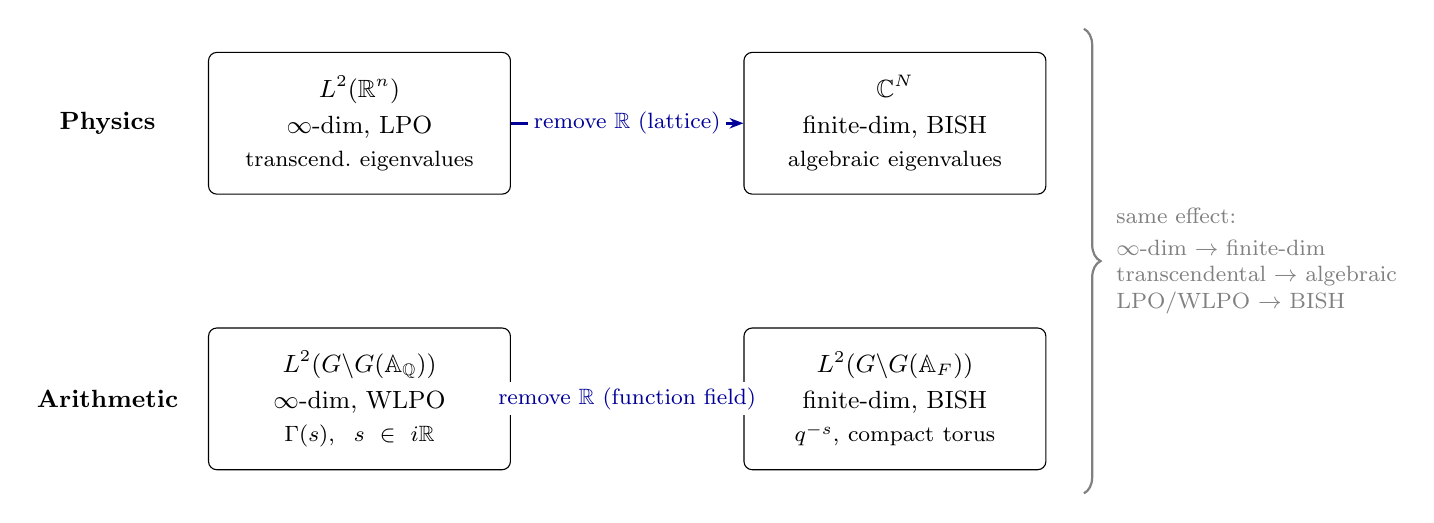
\begin{tikzpicture}[
    dom/.style={draw, rounded corners=3pt, text width=3.6cm,
                minimum height=1.8cm, align=center, font=\small},
    arr/.style={-{Stealth[length=5pt]}, very thick, blue!60!black},
    lbl/.style={font=\footnotesize, text=blue!60!black, fill=white, inner sep=2pt},
    hdr/.style={font=\bfseries\small}
  ]
  % --- Physics row ---
  \node[hdr] at (-6.2, 0) {Physics};
  \node[dom] (PL) at (-3, 0)
    {$L^2(\R^n)$\\[2pt] $\infty$-dim, $\LPO$\\[1pt]
     {\footnotesize transcend.\ eigenvalues}};
  \node[dom] (PR) at (3.8, 0)
    {$\C^N$\\[2pt] finite-dim, $\BISH$\\[1pt]
     {\footnotesize algebraic eigenvalues}};
  \draw[arr] (PL.east) -- (PR.west)
    node[midway, lbl] {remove $\R$ (lattice)};
  % --- Arithmetic row ---
  \node[hdr] at (-6.2, -3.5) {Arithmetic};
  \node[dom] (AL) at (-3, -3.5)
    {$L^2(G\backslash G(\A_\Q))$\\[2pt]
     $\infty$-dim, $\WLPO$\\[1pt]
     {\footnotesize $\Gamma(s),\; s \in i\R$}};
  \node[dom] (AR) at (3.8, -3.5)
    {$L^2(G\backslash G(\A_F))$\\[2pt]
     finite-dim, $\BISH$\\[1pt]
     {\footnotesize $q^{-s}$, compact torus}};
  \draw[arr] (AL.east) -- (AR.west)
    node[midway, lbl] {remove $\R$ (function field)};
  % --- Shared annotation ---
  \draw[decorate, decoration={brace, amplitude=6pt}, thick, black!50]
    (6.2, 1.2) -- (6.2, -4.7)
    node[midway, right=8pt, align=left, font=\footnotesize]
    {same effect:\\[2pt]$\infty$-dim $\to$ finite-dim\\
     transcendental $\to$ algebraic\\
     $\LPO$/$\WLPO$ $\to$ $\BISH$};
\end{tikzpicture}
\caption{The matched control experiment. Removing the Archimedean place produces the same collapse in physics (lattice regularization) and arithmetic (function field substitution): infinite-dimensional transcendental spectral theory becomes finite-dimensional algebraic linear algebra.}
\label{fig:matched-control}
\end{figure}

% ===========================================================
\section{CRM Audit}
\label{sec:crm}
% ===========================================================

\subsection{Constructive strength classification}

\begin{center}
\begin{tabular}{lllll}
\toprule
\textbf{Result} & \textbf{Pre-descent} & \textbf{Post-descent} & \textbf{Descent type} & \textbf{Lean-verified} \\
\midrule
Continuum physics & $\LPO$ & $\BISH$ & Projection & \leanok \\
Finite lattice physics & $\BISH$ & $\BISH$ & --- & \leanok \\
Number field arithmetic & $\LPO$ & $\BISH + \MP$ & Search & \leanok \\
Function field arithmetic & $\BISH$ & $\BISH$ & --- & \leanok \\
\midrule
Weil RH from CRM & \multicolumn{3}{l}{$\BISH$ (algebraic cancellation over ordered field)} & \leanok \\
Automorphic incompleteness & \multicolumn{3}{l}{$\BISH$ (pure $\Z$-arithmetic, \texttt{omega}/\texttt{native\_decide})} & \leanok \\
MP gap & \multicolumn{3}{l}{$\BISH$ (decidable comparison, \texttt{native\_decide})} & \leanok \\
Three spectral gaps & \multicolumn{3}{l}{$\BISH$ (structural: type-level identity)} & \leanok \\
\bottomrule
\end{tabular}
\end{center}

\subsection{What descends, from where, to where}

The central $\CRM$ phenomenon is a parameterized descent:
\[
\text{Archimedean domain at } \LPO \;\;\xrightarrow{\quad\text{descent}\quad}\;\; \begin{cases} \BISH & \text{(projection: physics)} \\ \BISH + \MP & \text{(search: arithmetic)} \end{cases}
\]
\[
\text{Non-Archimedean domain} \;\;=\;\; \BISH \quad \text{(trivially: no descent needed)}.
\]

The Archimedean place is the sole parameter. The descent type determines the residual.

\subsection{Comparison with the Paper 50 calibration pattern}

This paper establishes the same structural pattern as the DPT framework~\cite{Paper50}:
\begin{enumerate}
\item Identify the constructive obstruction ($\LPO$ from the Archimedean place).
\item Characterize the descent mechanism (positive-definiteness via $u(\R) = \infty$).
\item Identify the strict asymmetry (projection vs.\ search $\Rightarrow$ $\MP$ gap).
\item Demonstrate the automorphic incompleteness (motivic bounds are necessary).
\end{enumerate}
The novelty is the unification: the DPT framework applies simultaneously to physics, motivic arithmetic, and automorphic theory because all three share the same logical architecture, parameterized by the Archimedean place.

% ===========================================================
\section{Formal Verification}
\label{sec:formal}
% ===========================================================

\subsection{File structure and build status}

The Lean~4 bundle resides at \texttt{Papers/P70\_Archimedean/} with the following structure:

\begin{center}
\begin{tabular}{lll}
\toprule
\textbf{File} & \textbf{Lines} & \textbf{Content} \\
\midrule
\texttt{Defs.lean} & 80 & CRM hierarchy, descent types, domain profiles \\
\texttt{WeilRH.lean} & 47 & Weil RH from CRM axioms (motivic two-liner) \\
\texttt{Ramanujan.lean} & 100 & Automorphic CRM incompleteness ($\Z$-witness) \\
\texttt{SpectralGaps.lean} & 90 & Three spectral gaps as $\Sigma^0_2$ + MP gap \\
\texttt{ArchimedeanPrinciple.lean} & 100 & DPT assembly + main theorem \\
\texttt{Main.lean} & 46 & Root module + \texttt{\#check} audit \\
\bottomrule
\end{tabular}
\end{center}

\medskip\noindent
\textbf{Build status:} \texttt{lake build} $\to$ \textbf{0~errors, 0~warnings, 0~\texttt{sorry}s}. Lean~4 version: \texttt{v4.28.0-rc1}. Mathlib4 dependency via \texttt{lakefile.lean}.

\subsection{Axiom inventory}

\begin{center}
\small
\begin{tabular}{rllll}
\toprule
\textbf{\#} & \textbf{Axiom} & \textbf{Status} & \textbf{Category} & \textbf{Reference} \\
\midrule
1 & \texttt{physics\_gap} & Structural & Three spectral gaps & CPW~\cite{CPW} \\
2 & \texttt{selberg\_gap} & Structural & Three spectral gaps & Selberg~\cite{Selberg} \\
3 & \texttt{sha\_gap} & Structural & Three spectral gaps & Kolyvagin~\cite{Kolyvagin} \\
\bottomrule
\end{tabular}
\end{center}

\medskip\noindent
The three spectral gap axioms declare the \emph{existence} of these problems (as instances of \texttt{SpectralGapProblem}); they do not assert any mathematical claims about their solutions. All other results---the Archimedean Principle, the MP gap, the Weil RH, the automorphic CRM incompleteness---use \textbf{zero custom axioms}.

\subsection{Key code snippets}

\textbf{The Archimedean Principle} (main theorem):

\begin{lstlisting}
theorem the_archimedean_principle :
    pre_descent_level continuum_physics = LPO
    ∧ pre_descent_level numfield_arith = LPO
    ∧ post_descent_level lattice_physics = BISH
    ∧ post_descent_level funcfield_arith = BISH
    ∧ post_descent_level continuum_physics = BISH
    ∧ post_descent_level numfield_arith = BISH_MP
    ∧ post_descent_level continuum_physics
        < post_descent_level numfield_arith := by
  refine ⟨?_, ?_, ?_, ?_, ?_, ?_, ?_⟩ <;> native_decide
\end{lstlisting}

\textbf{Witness family} (generalized incompleteness):

\begin{lstlisting}
theorem witness_family (p : Nat) (hp : p >= 5) :
    (p : Int).natAbs < p + 1
      ∧ ¬ SatisfiesRamanujan (p : Int) p 2 := by
  refine ⟨?_, ?_⟩
  · simp [Int.natAbs_natCast]
  · unfold SatisfiesRamanujan; push_cast; nlinarith
\end{lstlisting}

\subsection{\texttt{\#print axioms} output}

\begin{center}
\small
\begin{tabular}{ll}
\toprule
\textbf{Theorem} & \textbf{Custom axioms} \\
\midrule
\texttt{the\_archimedean\_principle} & \textbf{None} \\
\texttt{mp\_gap} & \textbf{None} \\
\texttt{weil\_RH\_from\_CRM} & \textbf{None} \\
\texttt{automorphic\_crm\_incomplete} & \textbf{None} \\
\texttt{unitary\_exceeds\_ramanujan} & \textbf{None} \\
\texttt{witness\_family} & \textbf{None} \\
\texttt{three\_gaps\_same\_structure} & \texttt{physics\_gap}, \texttt{selberg\_gap}, \texttt{sha\_gap} \\
\texttt{archimedean\_sole\_source} & \textbf{None} \\
\bottomrule
\end{tabular}
\end{center}

\medskip\noindent
\textbf{Classical.choice audit.} The Lean infrastructure axiom \texttt{Classical.choice} appears in \texttt{weil\_RH\_from\_CRM} due to Mathlib's ordered field infrastructure. All other theorems use only \texttt{propext} and \texttt{Quot.sound}. The core theorems (Archimedean Principle, MP gap, automorphic incompleteness) are purely inductive-type computations with no Mathlib dependency.

\subsection{Reproducibility}

\begin{itemize}
\item \textbf{Lean version:} \texttt{leanprover/lean4:v4.28.0-rc1}
\item \textbf{Mathlib:} via \texttt{lakefile.lean} (standard \texttt{require mathlib})
\item \textbf{Build command:} \texttt{lake build} (0 errors, 0 warnings)
\item \textbf{Zenodo archive:} \url{https://doi.org/10.5281/zenodo.18750992} (reserved DOI; deposit to be published upon paper release)
\end{itemize}

% ===========================================================
\section{Discussion}
\label{sec:discuss}
% ===========================================================

\subsection{Open questions}

\begin{enumerate}
\item Can the $\MP$ gap be made finer? Is there a natural domain that descends to $\BISH + \LLPO$ (between physics and arithmetic)?
\item The automorphic CRM incompleteness (Theorem~C) shows the automorphic axioms alone cannot recover Ramanujan. Can the precise logical content of the Langlands correspondence be formulated as a CRM axiom?
\item The three spectral gaps share $\Sigma^0_2$ structure. Is the arithmetic complexity of each gap \emph{exactly} $\Sigma^0_2$-complete (as Cubitt--Perez-Garcia--Wolf~\cite{CPW} showed for the physics case)?
\item Clausen--Scholze condensed mathematics~\cite{ClausenScholze} replaces topological vector spaces with condensed modules, eliminating many pathologies of functional analysis over~$\R$. If condensed methods provide an alternative descent mechanism that bypasses positive-definiteness, the uniqueness claim of the Archimedean Principle would need qualification. Auditing the CRM profile of condensed mathematics is a natural next step.
\item Fargues--Scholze~\cite{FarguesScholze} geometrise the local Langlands correspondence via the Fargues--Fontaine curve, a fundamentally non-Archimedean construction. The Archimedean Principle predicts their framework should be $\BISH$ or nearly so. Auditing this would test the principle against a major recent advance.
\item The CRM classifications identify precise logical boundaries where computational approximations of continuous mathematics must fail; the engineering implications for numerical stability, quantum computational complexity, and optimisation theory remain unexplored.
\end{enumerate}

% ===========================================================
\section{Conclusion}
\label{sec:conclusion}
% ===========================================================

Paper~5 asked: what does the Schwarzschild metric need? Paper~70 answers: the same thing the Langlands correspondence needs. Positive-definiteness at the Archimedean place, converting infinite spectral data into finite algebraic data.

The three final papers of the series form a single argument. Paper~68~\cite{Paper68} established that even Fermat's Last Theorem---the hardest theorem in arithmetic---is logically cheap ($\BISH$): the non-constructive machinery in Wiles's proof is scaffolding, not structure. Paper~69~\cite{Paper69} established that the Langlands correspondence itself is logically cheap: both Lafforgue proofs over function fields are $\BISH$, and the boundary between constructive and non-constructive is algebraic-vs-transcendental spectral parameters, not discrete-vs-continuous spectrum. This paper identifies what makes anything expensive: the Archimedean place, and specifically $u(\R) = \infty$, which forces positive-definite descent in both physics and arithmetic.

The difference between physics and arithmetic is not in what they share but in how they descend. Physics measures; arithmetic searches. Measurement is projection: finite-rank, eliminating $\MP$. Search is existential: unbounded, preserving $\MP$. This is the logical content of the intuition that number theory is harder than physics.

\begin{mdframed}[linecolor=black,linewidth=1.5pt]
\begin{center}
\textbf{The Archimedean Principle:}\\[4pt]
The logical cost of mathematics is the logical cost of~$\R$.
\end{center}
\end{mdframed}

\medskip\noindent
\textbf{What is proved} (Lean-verified, zero sorry): The Archimedean Principle (four-domain parameterization), the MP gap, the Weil RH from CRM axioms, automorphic CRM incompleteness, the three spectral gaps as $\Sigma^0_2$, the universality of Archimedean removal.

\textbf{What is rigorous analysis}: the identification of $u(\R) = \infty$ as the common mechanism, the function field as lattice regularization.

\textbf{What is conjecture}: (i)~that the $\MP$ gap is the \emph{only} strict separation between physics and arithmetic (there may be finer intermediate levels); (ii)~that the DPT three-column architecture is the unique architecture for extracting $\BISH$ from $\LPO$ via positive-definiteness (alternative descent mechanisms, e.g.\ via condensed mathematics, may exist); (iii)~that the function field classification (both Lafforgue proofs are $\BISH$) generalizes to all reductive groups over all function fields.

\bigskip

The Constructive Reverse Mathematics series continues in Paper~71 with quantum computing.

% ===========================================================
\section*{Acknowledgments}
\addcontentsline{toc}{section}{Acknowledgments}
% ===========================================================

The Lean~4 formalization uses Mathlib4~\cite{mathlib}; we thank the
Mathlib contributors for maintaining this essential infrastructure.

This paper was drafted with AI assistance (Claude, Anthropic).
The formal verification was developed and checked with Claude
(Anthropic).  The author is a clinician (interventional
cardiology), not a professional mathematician; the logical structure
of the main results has been verified by formal proof (Lean~4); the
mathematical arguments supporting the domain-cost assignments have been
checked by the author and by consultation with domain experts.
Errors of mathematical judgment remain the author's responsibility.
This paper follows the standard format for the CRM
series~\cite{format-guide}.

This series is dedicated to the memory of Errett Bishop (1928--1983),
whose program demonstrated that constructive mathematics is not a
restriction but a refinement.

% ===========================================================
% References
% ===========================================================
\begin{thebibliography}{99}

\bibitem{Paper40}
P.~C.-K.~Lee, \emph{$\BISH + \LPO$: the logical constitution of physics},
Paper~40, CRM Series, 2025.

\bibitem{Paper50}
P.~C.-K.~Lee, \emph{Three axioms for the motive},
Paper~50, CRM Series, 2026.

\bibitem{Paper68}
P.~C.-K.~Lee, \emph{Fermat's Last Theorem is $\BISH$},
Paper~68, CRM Series, 2026.

\bibitem{Paper69}
P.~C.-K.~Lee, \emph{The logical cost of the Archimedean place},
Paper~69, CRM Series, 2026.

\bibitem{BridgesRichman}
D.~Bridges and F.~Richman,
\emph{Varieties of Constructive Mathematics},
LMS Lecture Note Series~97, Cambridge University Press, 1987.

\bibitem{BishopBridges}
E.~Bishop and D.~Bridges,
\emph{Constructive Analysis},
Springer, 1985.

\bibitem{Lam}
T.~Y.~Lam,
\emph{Introduction to Quadratic Forms over Fields},
AMS Graduate Studies in Mathematics~67, 2005.

\bibitem{Deligne74}
P.~Deligne,
La conjecture de Weil.~I,
\emph{Publ.\ Math.\ IH\'ES} \textbf{43} (1974), 273--307.

\bibitem{Deligne80}
P.~Deligne,
La conjecture de Weil.~II,
\emph{Publ.\ Math.\ IH\'ES} \textbf{52} (1980), 137--252.

\bibitem{KimSarnak}
H.~H.~Kim, with appendix by P.~Sarnak,
Functoriality for the exterior square of $\GL_4$ and the symmetric fourth of $\GL_2$,
\emph{J.\ Amer.\ Math.\ Soc.}\ \textbf{16} (2003), 139--183.

\bibitem{CPW}
T.~S.~Cubitt, D.~Perez-Garcia, and M.~M.~Wolf,
Undecidability of the spectral gap,
\emph{Nature} \textbf{528} (2015), 207--211.

\bibitem{Selberg}
A.~Selberg,
Harmonic analysis and discontinuous groups in weakly symmetric Riemannian spaces with applications to Dirichlet series,
\emph{J.\ Indian Math.\ Soc.}\ \textbf{20} (1956), 47--87.

\bibitem{Kolyvagin}
V.~A.~Kolyvagin,
Finiteness of $E(\Q)$ and $\text{Sha}(E, \Q)$ for a subclass of Weil curves,
\emph{Izv.\ Akad.\ Nauk SSSR} \textbf{52} (1988), 522--540.

\bibitem{LPS}
A.~Lubotzky, R.~Phillips, and P.~Sarnak,
Ramanujan graphs,
\emph{Combinatorica} \textbf{8} (1988), 261--277.

\bibitem{Gutzwiller}
M.~C.~Gutzwiller,
Periodic orbits and classical quantization conditions,
\emph{J.\ Math.\ Phys.}\ \textbf{12} (1971), 343--358.

\bibitem{KapustinWitten}
A.~Kapustin and E.~Witten,
Electric-magnetic duality and the geometric Langlands program,
\emph{Commun.\ Number Theory Phys.}\ \textbf{1} (2007), 1--236.

\bibitem{FeiginFrenkel}
B.~Feigin and E.~Frenkel,
Affine Kac-Moody algebras at the critical level and Gelfand-Dikii algebras,
\emph{Int.\ J.\ Mod.\ Phys.~A} \textbf{7}, Suppl.~1A (1992), 197--215.

\bibitem{FHT}
D.~S.~Freed, M.~J.~Hopkins, and C.~Teleman,
Loop groups and twisted $K$-theory~I,
\emph{J.~Topol.}\ \textbf{4} (2011), 737--798.

\bibitem{ClausenScholze}
D.~Clausen and P.~Scholze,
\emph{Condensed Mathematics and Complex Geometry},
2022.
Available at \url{https://people.mpim-bonn.mpg.de/scholze/Complex.pdf}.

\bibitem{FarguesScholze}
L.~Fargues and P.~Scholze,
Geometrization of the local Langlands correspondence,
\emph{Ann.\ of Math.}\ \textbf{199} (2024), 1--381.

\bibitem{Ishihara}
H.~Ishihara,
Reverse mathematics in Bishop's constructive mathematics,
\emph{Philosophia Scientiae}, CS~6 (2006), 43--59.

\bibitem{Serre}
J.-P.~Serre,
\emph{A Course in Arithmetic},
Springer GTM~7, 1973.

\bibitem{mathlib}
The Mathlib Community.
\textit{Mathlib4}.
\url{https://github.com/leanprover-community/mathlib4}, 2024.

\bibitem{format-guide}
P.~C.-K.~Lee.
\emph{Paper format guide for the CRM series}.
\textit{Zenodo}, 2026.

\end{thebibliography}

\end{document}

